\input{../YKY-preamble}

\usepackage{hyperref}		% include web link for RL sample code

\definecolor{Cerulean}{RGB}{100,100,200}
\newcommand{\emp}[1]{\textbf{\textcolor{Cerulean}{#1}}}

\newsavebox{\MyName}
\savebox{\MyName}{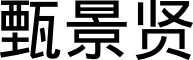
\includegraphics[scale=0.6]{YKY.png}}

\title{强化学习 tutorial}
%\titlerunning{强化学习 tutorial}
\author{\usebox{\MyName} (King-Yin Yan)
\\ \footnotesize{General.Intelligence@Gmail.com}
}
%\institute{General.Intelligence@Gmail.com}

\begin{document}

\maketitle
\setlength{\parindent}{0em}
% \setlength{\parskip}{2.8ex plus0.8ex minus0.8ex}
\setlength{\parskip}{2.8ex}

%\begin{abstract}
%简单介绍强化学习。
% 假设 $x$ 是思维状态。 在经典逻辑智能中,$x$ 是一束命题,代表当下的思考状况。 思考的过程就是不断重复进行推导: $x \vdash x' \vdash ...$。 在经典 AI 中这个作用是靠无数的逻辑 rules 来达成的。 但现在我们的做法是将 $x$ 放到向量空间中,再用一个 recurrent 神经网络来取代整个 rules base。
%\end{abstract}

\section{什么是强化学习?}

Reinforcement learning 是机器学习里面的一个分支,特别善於控制一只能够在某个环境下 \emp{自主行动} 的个体 (autonomous agent),透过和 \emp{环境} 之间的互动,例如 sensory perception 和 rewards,而不断改进它的 \emp{行为}。

听到强化学习,你脑里应该浮现一只曱甴那样的小昆虫,那就是 autonomous agent 的形象:
\begin{equation}

\includegraphics[scale=0.2]{cockroach.png}
\end{equation}

对「环境」(environment) 这概念,你应该想到像以下这经典游戏的迷宫:
\begin{equation}
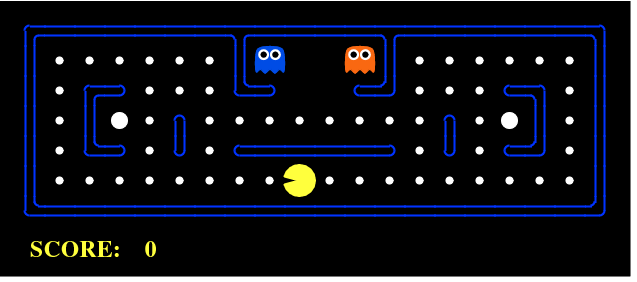
\includegraphics[scale=0.8]{pacman-0.png}
\end{equation}

包括有追捕你的怪物、和吃了会加分的食物 (这些代表负值和正值的 rewards)。  当然,实际应用的「环境」和「奖励」可以是抽象的,这游戏是一个很具体的例子。

\subsection{输入/输出}

记住,reinforcement learning 的 \emp{输入} 是:
\let\labelitemi\labelitemii
\begin{itemize}
\item 状态 (States) = 环境,例如迷宫的每一格是一个 state
\item 动作 (Actions) = 在每个状态下,有什么行动是容许的
\item 奖励 (Rewards) = 进入每个状态时,能带来正面或负面的 价值 (utility)
\end{itemize}
而输出就是:
\begin{itemize}
\item 方案 (Policy) = 在每个状态下,你会选择哪个行动?
\end{itemize}
於是这 4 个元素的 tuple $(S,A,R,P)$ 就构成了一个强化学习的系统。   在抽象代数中我们常常用这 tuple 的方法去定义系统或结构。

再详细一点的例子就是:
\begin{itemize}
\item states $S$ = 迷宫中每一格的位置,可以用一对座标表示,例如 (1,3)
\item actions $A$ = 在迷宫中每一格,你可以行走的方向,例如: $\{$ 上,下,左,右 $\}$
\item rewards $R$ = 当前的状态 (current state) 之下,迷宫中的那格可能有食物 (+1) 、也可能有怪兽 (-100)
\item policy $P$ = 一个由 状态 $\rightarrow$ 行动 的 函数,意即: 这函数对给定的每一个状态,都会给出一个行动。 
\end{itemize}
$(S, A, R)$ 是使用者设定的, $P$ 是算法自动计算出来的。  

\subsection{人与虫之间}

第一个想到的问题是: 为什么不用这个方法打造人工智能?  但现时的强化学习算法,只对比较细小和简单的环境适用,对於大的复杂的世界,例如象棋的 $10^{\mbox{xxx}}$ 状态空间,仍是 intractable 的。

关键就是,高等智慧生物会在脑中建立世界的模型 (world model) 或知识 (knowledge), 而强化学习只是关心简单的「状态-行动」配对。

强化学习的领导研究者 Richard Sutton 认为,只有这种学习法才考虑到 自主个体、环境、奖励 等因素,所以它是人工智能中最 top-level 的 architecture,而其他人工智能的子系统,例如 logic 或 pattern recognition,都应该在它的控制之下,我觉得颇合理。
\begin{equation}
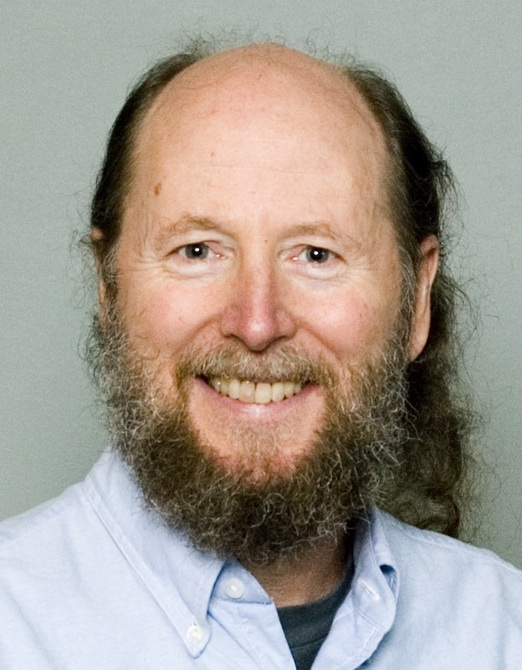
\includegraphics[scale=0.4]{Richard-Sutton.jpg}
\end{equation}

所以要制造 strong AI,一个可能的方案就是结合强化学习和某种处理复杂 world model 的能力:
\begin{equation}
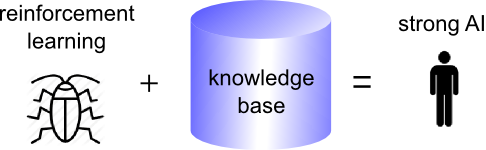
\includegraphics[scale=0.7]{cockroach-KB-person.png}
\end{equation}

\noindent 「\textit{你们已经由虫进化成人,但在你们之内大部份仍是虫。}」

\hfill --- 尼采, Thus spoke Zarathustra

\noindent 「\textit{如果人类不相信他们有一天会变成神,他们就肯定会变成虫。}」

\hfill --- Henry Miller

%\begin{comment}
% ===========================================================================
\subsection{程式}

学 AI 最紧要有 program,不然就会很枯燥。  这是我在网上找到的一个特别简单的 demo,作者是 Travis DeWolf:

\href{https://studywolf.wordpress.com/2012/11/25/reinforcement-learning-q-learning-and-exploration/}{Reinforcement learning demo}

只要 Python 便可运行,但你可能要 install PyGame。

猫、老鼠、芝士:
\begin{equation}
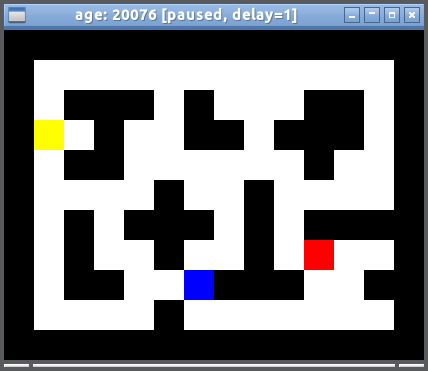
\includegraphics[scale=0.25]{RL-demo.png}
\end{equation}

猫的行动是简单地朝着老鼠追(没有智能),老鼠的行动是学习出来的。

注意,在 main program 和 cellular.py 这两部分,纯粹是定义了迷宫世界如何运作,基本上是一个 game,里面完全没有智能,你可以用{上、下、左、右} 控制各 agent 的活动,如此而已。

强化学习的程式在 qlearn.py,很短,而真正学习的程式基本上只有一句,就是:

\tab \code{def learnQ(self, state, action, reward, value): }\\
\tab \code{oldv = self.q.get((state, action), None) }\\
\tab \code{if oldv is None:} \\
\tab \code{\tab self.q[(state, action)] = reward }\\
\tab \code{else: }\\
\tab \code{\tab \textcolor{red}{self.q[(state, action)] = oldv + self.alpha * (value - oldv) }}

单是这一句程式,就能令老鼠学到避开猫、吃芝士。  以下再解释....

% ===========================================================================
%\end{comment}

\subsection{強化學習的原理}

《AI-a modern approach》这本书第 21 章有很好的简介。  《AIMA》自然是经典,很多人说他们是读这本书而爱上 AI 的。  这本书好处是,用文字很耐性地解释所有概念和原理,思路很清晰,使读者不致有杂乱无章的感觉。  例如 21 章 首先讲 passive reinforcement learning,意思是当 policy 是固定时,纯粹计算一下 agent 期望的价值(utility,即 rewards 的总和) 会是多少。  有了这基础后再比较不同 policies 的好坏。  这种思路在数学中很常见: 首先考虑简单到连白痴也可以解决的 case,然后逐步引入更多的复杂性。  例如数学归纳法,由 $N=1$ 的 case 推到 $N \rightarrow \infty$。

为免重复,我只解释到明白 $Q$ learning 的最少知识。

\subsection{Utility (价值,或效)}

$U$ 是一连串行动的 rewards 的总和。  例如说,行一步棋的效用,不单是那步棋当前的利益,还包括走那步棋之后带来的后果。  例如,当下贪吃一只卒,但 10 步后可能被将死。  又或者,眼前有美味的食物,但有些人选择不吃,因为怕吃了会变肥。

一个 state 的效用 U 就是: 假设方案固定,考虑到未来所有可能的 transitions,从这个 state 开始的平均期望的 total reward 是多少 :

$$ U(S_0) = \mathbb{E}[ \; \sum_{t=0}^{\infty} \; \gamma^t \; R(S_t) \; ] $$

其中 $\mathbb{E[\;]}$ 代表期望值,$\gamma$ 是 discount factor,例如 0.9 或什么。

实例: 考虑这简单的迷宫:
\begin{equation}
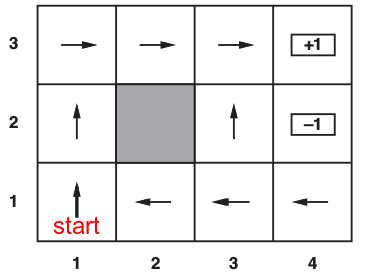
\includegraphics[scale=0.4]{RL-simple-maze.png}
\end{equation}

那些箭咀表示的是众多可能方案中的其中一个。

根据这个方案,由 $(1, 1)$ 开始的运行可能是这个结果:
\begin{equation}
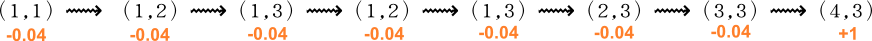
\includegraphics[scale=0.7]{RL-state-transition-eg-1.png}
\end{equation}

下面橙色的值是每个 state 的 reward。  在这例子中,每个不是终点的格,也会扣 0.04 分。

但从同一起点,同一方案,也可以出现不同结果,例如在 (1,3) 企图向右爬,但实际结果是向下跌一格; 这些 state transitions 是由外在世界的机率决定的。  (例如某人读了大学文凭,但遇上经济不景,他的薪水未必能达到行动的预期效果。)

同一方案的运行结果可以是:
\begin{equation}
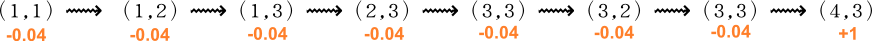
\includegraphics[scale=0.7]{RL-state-transition-eg-2.png}
\end{equation}
或者:
\begin{equation}
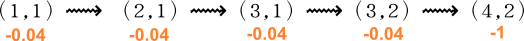
\includegraphics[scale=0.7]{RL-state-transition-eg-3.png}
\end{equation}

\subsection{Bellman condition}

这是 dynamic programming(动态规划)的中心思想,又叫 Bellman optimality condition。

在人工智能里我们叫 reinforcement learning,但在控制论的术语里叫 dynamic programming,两者其实是一样的。 Richard Bellman 在 1953 年提出这个方程,当时他在 RAND 公司工作,处理的是运筹学的问题。 他也首先使用了 "curse of dimensionality" 这个术语,形容动态规划的主要障碍。

考虑的问题是: 要做一连串的 sequential decisions。

Bellman equation 说的是: 「\textbf{如果从最佳选择的路径的末端截除一小部分,馀下的路径仍然是最佳路径。}」

换句话说,如果一系列的选择 A B C D E.... 是最优的,那么这系列除去开始的 A,那 B C D E.... 系列应用在后继的状态上也是最优的。

(例如,你从香港乘车到北京,选择了最便宜的路线,此路线经过 10 个车站,第二站是深圳:
$$ \mbox{香港} \rightarrow \mbox{深圳} \rightarrow ... ... \rightarrow \mbox{北京} $$
但如果除去出发点香港站,那么由第二站深圳到最后的北京站:
$$ \mbox{深圳} \rightarrow ... ... \rightarrow \mbox{北京} $$
这路线仍然是馀下 9 个站之间最便宜的。)

用数学表示:
$$ U^*(S) = \max_a \{ R(a) + U^*(S') \} $$
$$ \mbox{ie,} \quad \quad U^*(\mbox{全路径}) = \max_a \{ R(\mbox{在当前状态下选取 a}) + U^*(\mbox{馀下路径}) \} $$
$*$ 表示 \emp{最优} (optimal)。 这条看似简单的式子是动态规划的全部内容; 它的意义是: 我们想获得最佳效益的路径,所以将路径切短一些,於是问题化解成一个较小的问题;  换句话说它是一个 recursive relation。

\subsection{Delta rule}

这只是一个简单的 trick,在机器学习中经常出现。  假设我们有一个理想,我们要逐步调教当前的状态,令它慢慢趋近这个理想。 方法是: 
$$ \mbox{当前状态} := \mbox{当前状态} + \alpha ( \mbox{理想} - \mbox{当前状态}) $$
其中 $\alpha$ 叫「学习速度 (learning rate)」。 "Delta" ($\Delta$) 指的是理想和现状之间的差异。

很明显,只要反覆执行上式,状态就会逐渐逼近理想值。

(Delta rule 的微分形式就是我们熟悉的「梯度下降」: $x \mbox{ += } \eta \cdot \frac{dy}{dx}$)

\subsection{Temporal difference (TD) learning}

将 delta rule 应用到 Bellman condition 上,去寻找最优路径,这就是 temporal difference learning。

我们还是从简单情况开始:  假设方案固定,目标是学习每个 state 的 utility。

理想的 $U(S)$ 值,是要从 state $S$ 开始,试验所有可能的 transitions,再计算这些路径的 total rewards 的平均值。

但实际上,agent 只能够每次体验一个行动之后的 state transition。

所以要应用 Bellman condition: 一个 state $S$ 的 $U$ 值,是它自身的 reward,加上所有可能的后继 states 的 $U$ 值,取其机率平均,再乘以 discount factor $\gamma$:
$$ U(S) = R(S) + \gamma \sum_{S'} P(S \rightarrow S') \; U(S') $$
其中 $P$ 是 transition 的机率,$S'$ 是后继 state,$\sum$ 是对所有后继 states 求和。  换句话说,这是理想的 $U(S)$ 和 $U(S \mbox{的后继})$ 之间的关系,是一个 recursive relation。

例如,假设 agent 现时对 state (1,3) 和 state (2,3) 的估值,分别为 0.84 和 0.92。  又假设 agent 察觉到,根据现有方案,在 (1,3) 时总是会发生跳到 (2,3) 这个 transition。  那么这两个 states 的 $U$ 值,应该符合这条约束:
$$ U(1,3) = -0.04 + U(2,3) $$
换句话说,这是两个 states 之间,U 值的 local (局部的)约束。

TD learning 的思想是:  假设其他 $U(S')$ 的值正确,利用 Bellman optimality 来调整当下 state 的 $U(S)$。 当尝试的次数多了,所有 $U$ 值都会趋向理想。 Agent 只需要用这条 update rule:
$$ U(S) \mbox{  +=  } \alpha [ \; R(S) + \gamma U(S') - U(S) \; ] $$

$\alpha$ 是 learning rate,它决定学习的速度(但它不能太大,避免 overshooting)。  后面那东西是 $U(S)$ 和 $U(S)$ 的估值 (estimation) 之间的差别。  对於理想的 $U(S)$ 和 $U(S')$,那差别会是 0。  而在每个 time step,我们只是用 $\alpha$ 部分地 调整这个差别。

最后一提,在上面理想约束的公式里,有对於机率 P 的求和,但在 update formula 中 $P$ 不见了。  那是因为 agent 在环境中的行动,暗含了对於 state transition 机率的 sampling (随机地取样本)。 换句话说,那机率求和是由 agent 本身体现的。

$P$ 是 state transitions 的机率,换句话是关於世界的一个 model。 TD learning 不需要学习 $P$,所以叫 model-free learning。  但正如开篇时说过,model-free 并不一定是好事,人的智慧就是基於我们对外在世界有一些很好的 models。

\subsection{Q value}

$Q$ 值只是 $U$ 值的一个变种 ;   $U$ 是对每个 state 而言的,$Q$ 把 $U$ 值分拆成每个 state 中的每个 action 的份量。  换句话说,$Q$ 就是在 state $S$ 做 action $A$ 的 utility。

$Q$ 和 $U$ 之间的关系是:
$$ U(S) = \max_A  Q(S, A) $$

$Q$ 的好处是什么?  下面将会介绍 active learning,而 $Q$ value  配合 TD learning,可以在 active learning 中也消除 $P$,达到 model-free 的效果。

上面的 update rule 只要用这个关系改写就行:
$$ Q(S, A) \mbox{  +=  } \alpha [ \; R(S) + \gamma \max_{A'}  Q(S', A') - Q(S, A) \; ] $$

\subsection{Active learning}

在 passive learning 中,方案不变,我们已经能够计算每个 state $S$ 的效用 $U(S)$,或者每个 state $S$ 之下行动 $A$ 的效用 $Q(S, A)$。

如果方案是可以改变的,我们只需计算不同方案的 $Q$ 值,然后在每个 state $S$ 选取相应於最大 $Q$ 值的行动 $A$,那就是最佳方案,不是吗?

实际上执行的结果,却发现这些 agent 的方案很差!  原因是,学习过程中的 $Q$ 值是 estimate,不是理想的 $Q$ 值,而如果根据这样的 $Q$ 行动,agent 变得很短视,不会找到 optimal policy。  (例如,某人经常吃同一间餐馆,但循另一路径走,可以发现更好的餐馆。)

Agent 需要尝试一些未知的状态/行动,才会学到 optimal policy;  这就是所谓的 exploration vs exploitation (好奇心 vs 短暂贪婪)之间的平衡。

方法是,人工地将未知状态的价值增加一点:
$$ U(S) = R(S) + \gamma \max_A \mathcal{F}[ \; \sum_{S'} P(S \rightarrow S') U(S'), \; N(S, A) \; ] $$
其中 $N(S, A)$ 是状态 $S$ 和行动 $A$ 这对组合出现过(被经历过)的次数,$\mathcal{F}$ 是 exploration 函数,它平时回覆正常的 $U$ 的估计值,但当 $N$ 很小时(亦即我们对 $S$,$A$ 的经验少),它会回覆一个比较大的估值,那代表「好奇心」的效用。

% 结语

% 本来想写一篇人人能读懂的 RL 简介,但发觉写到长篇大论才勉强解释完。  希望女朋友能读懂 :)

%\bibliographystyle{plain} % or number or aaai ...

\end{document}
